\documentclass[10pt]{article}
\usepackage{amsmath,amsfonts,amsthm,amssymb}
\usepackage{fancyhdr}
\usepackage{chngpage}
\usepackage{color}
\usepackage{boxedminipage}
\usepackage{pbox}
\usepackage{lscape}

\usepackage{graphicx}
\usepackage{watermark}
\thiswatermark{\centering \put(0,-500){
\includegraphics[scale=1.5]{goshawk1.eps}} }


\title{GosHawk - Smart App \\ Documatation}
\author{Itay Parnafes \& Tomer Shalmon}

\begin{document}

\maketitle
\date
\newpage
\tableofcontents
\newpage
\section{Introduction}
GosHawk is a smart compact home security system based on open-source development platforms. \\
GosHawk was built and designed to be as simple as possible so that the ordinary user can set it up and use it without any previous knowledge. \\
The GosHawk mobile app strives to be as user-friendly as possible in order to provide an easy convenient user experience. 
\\ \\
The current version of GosHawk is an alpha version, designated to provide a proof-of-concept for a free open-source modular smart home security system, initially started as a graduation project for computer-science bachelor degree.

\newpage
\section{System Architecture}
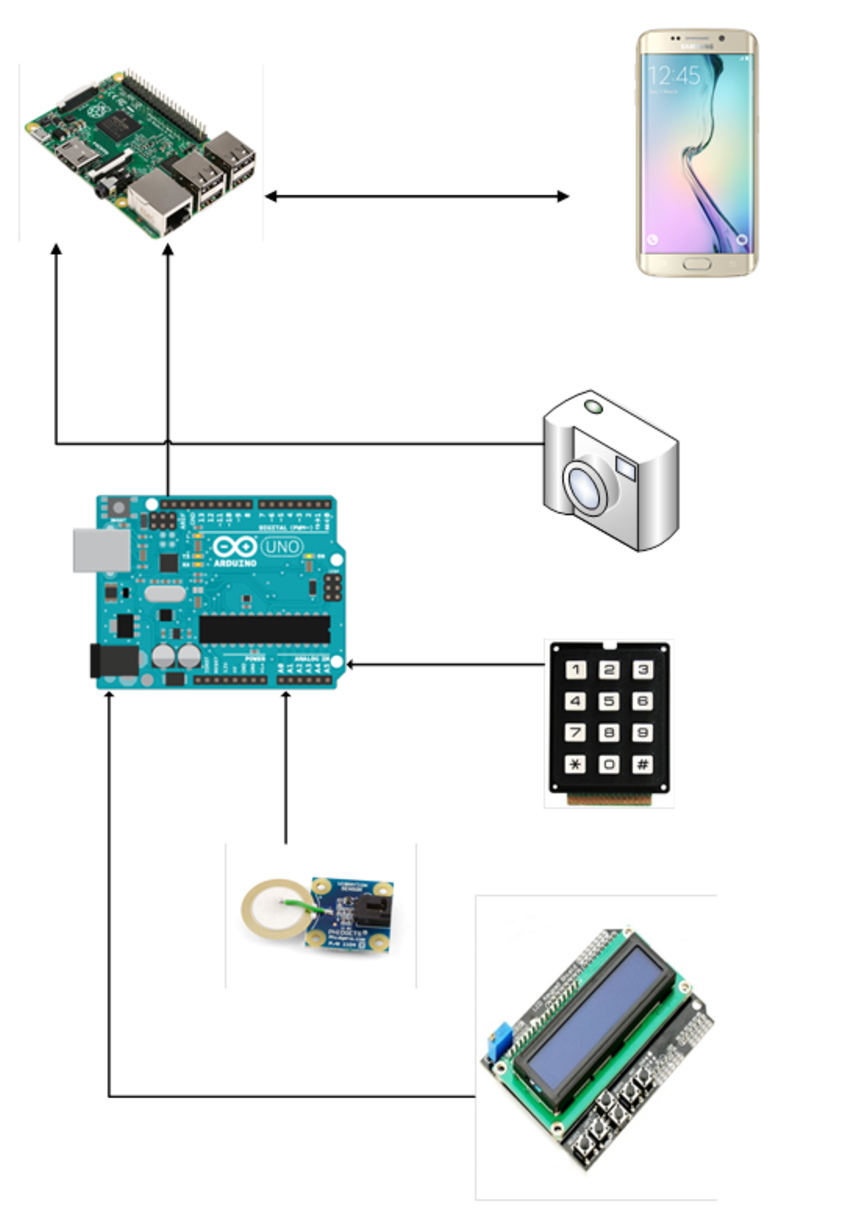
\includegraphics[scale=0.5]{arc.eps}
\subsection{Backend}
\subsubsection{Arduino}
Arduino is an open-source hardware, software and microcontroller based development board.
The specific type used in GosHawk is \emph{Arduino Uno}.
The Arduino is fed from different sensors scattered around the house, analyses its inputs and synchronizes with the main server.
The arduino uses an ethernet shield\footnote{Another board assembled on top of the main board in order to provide ethernet based communication.} in order to communicate with the main server using \emph{UDP}\footnote{User Datagram Protocol - Transport layer contectionless protocol used to deliver messages over IP network.} over port 9898\footnote{By default. Can be configured differently.}.
\\ \\
\quad The Arduino code is written in \emph{C++} and is well commented in order to provide highly detailed code for other coders to integrate their own code.
\\ \\Current supported sensors are described in details in section \ref{ss_sensors}.

\subsubsection{Sensors} \label{ss_sensors}
The system sensors were particulary chosen to give the maximum information on the house state in minimum cost. \\
The sensors has to be connected to the designated ports in order to work. \\ \\
\begin{tabular}{| l | l | l | l |}
	\hline
	\textbf{Sensor} & \textbf{Analog/Digital} & \textbf{I/O} & \textbf{Description} \\ \hline
	Keypad & Digital & Input & Keypad used to input local pincode \\ \hline
	Vibration sensor & Analog & Input & Detects vibrations on the door \\ \hline
	LCD Screen & Digital & Output & Displays key strokes on the keypad \\ \hline

\end{tabular}
\subsubsection{GoServer}
The server is the "heart" of the system and is in charge of communicating and synchronizing between all system components.
The server runs on a \emph{Raspberry Pi 2 Model B}\footnote{A credit card-sized single-board computer.} hardware running \emph{Ubuntu 16.04 Xential Server} operating-system. \\
The server runs several component, overwatched by a \emph{watchdog}\footnote{A process which runs using crontab and keeps all specified processes up and running.}. \\
\quad \subsubsection*{Synchronizer}
\quad A simple server which listens on UDP port 9898 and receives event messages from the \emph{Arduino} and updates the shared DB\footnote{Database}. \\
\quad The synchronizer was written in Python 2.7. \\
\quad \subsubsection*{Web Server}
\quad The web server is the main component of the GoServer and is designed to synchronize with the frontend components. \\
\quad The web server is designed to work solely with \emph{Android} clients\footnote{Currently iOS/web clients are not supported}, and provides fully integrated web app. \\
\quad The web server main jobs are:
\begin{itemize}
	\item Manage users registration and permissions
	\item Query shared DB as a backend component for the app
	\item Keep track of clients queries
	\item Arm and Disarm the system
	\item Check home presence of registered users
\end{itemize}
\quad The web server was written in \emph{Django}\footnote{Free and open-source web framework, written in Python, which follows the model–view–controller (MVC) architectural pattern.} 1.8.7 based on Python 2.7.

\quad \subsubsection*{Hawk-Eye}
\quad The Hawk-Eye is a python script used to take photos using the installed camera in the event of a breach. \\
\quad The Hawk-Eye was written in Python 2.7.


\subsection{Frontend}
\subsubsection{Android App}
blah blah blah....
\newpage
\section{Requirements}
\begin{itemize}
	\item Arduino (Uno or other)
	\item Ethernet shield
	\item Keypad
	\item Small LCD screen
	\item Vibrations sensor
	\item Raspberry Pi
	\item Foscam IP Camera\footnote{Any model}
\end{itemize}
\subsection{Raspberry Pi}
\begin{itemize}
	\item Ubuntu 16.04 Xenial Server
	\item Python 2.7	
	\item Django 1.8.7
	\item Nmap\footnote{Network Mapper}
	\item GoServer package
	\item Active internet connection
\end{itemize}

\section{System Components}
\subsection{Web Server}
As mentioned before - the web server is the "heart" of the system and is intermediating between the clients and the data layer such as events, images, etc. \\ 
Under the \emph{GoServer} main directory, the application files are located under \emph{app} directory. \\
\begin{itemize}	
	\item The database tables definitions and declarations are located in \emph{models.py}
	\item The url paths are located in \emph{urls.py}
	\item The methods actual implementation are located in \emph{views.py}
	\item All utility methods are located in \emph{utils.py}
\end{itemize}
The server listens by default to port TCP/8888 from all available interfaces. \\
The path from which the server is searching for captured pictures can be changed and is located in \emph{utils.py} under \emph{IMAGE\_PATH}. \\
All availble methods can be found in section \ref{sss_methods}. \\
\\ The web-server also provides a convenient admin control panel which provides advanced users a way to visually inspect and maintain server administrators and databse. \\
The admin contorl panel can be accessed via: \underline{http://goserver.address:8888/admin}. \\
\subsubsection{Server Available Methods} \label{sss_methods}
\begin{table}[ht]
\centering    
    \resizebox{\textwidth}{!}{\begin{tabular}{| l | l | l | p{3cm} | p{6.5cm} | l |}
      \hline
      \textbf{URI} & \textbf{Type} & \textbf{Parameters} & \textbf{Description} & \textbf{Response} & \textbf{Remarks} \\ \hline
      /app/login & POST & \pbox{30cm}{name \\ password} & A registered user login page & \pbox{25cm}{\{ \\
      'Access Granted': 'True',\\ 'uid': user\_id,\\ 'user\_type': permission \\ \}} & Cookies must be enabled \\ \hline
     /app/register\_mac & POST & mac & Register given mac to a registered user &\{'Success': 1\} & MAC address should be colon separated \\ \hline    
    /app/sync & GET & None & Request all unread events (by a specific user) & \pbox{25cm}{\{ \\ 
             	\quad events: [ \\ 
             		\qquad \{ \\ 
             		\qquad \quad "id": "862", \\
             			\qquad \quad timestamp: \{ \\ 
             				\qquad \quad \quad "hour": 7, \\ 
       					    \qquad \quad \quad "month": 3, \\ 
                            \qquad \quad \quad "second": 57, \\ 
             				\qquad \quad \quad "year": 2016, \\ 
             				\qquad \quad \quad "day": 5, \\ 
             				\qquad \quad \quad "minute": 48 \\ 
             			\qquad \quad \}, \\ 
             			\qquad \quad "type": "Breach", \\ 
             			\qquad \quad "description": "house has been breached", \\ 
             			\qquad \quad "severity": "Critical" \\ 
             		\qquad \quad \} \\ 
             	\qquad ] \\ 
             \quad \} \\
           } & \\ \hline
     /app/create\_new\_user & POST & \pbox{25cm}{name \\ password \\ permission} & Add new user to the local system & \{'Success': 1\} & Only 'Admin' can add new users \\ \hline
     /app/get\_recent\_events & GET & None & Reuqest 10 most recent system events & \pbox{25cm}{\{ \\ 
             	\quad events: [ \\ 
             		\qquad \{ \\ 
             		\qquad \quad "id": "862", \\
             			\qquad \quad timestamp: \{ \\ 
             				\qquad \quad \quad "hour": 7, \\ 
       					    \qquad \quad \quad "month": 3, \\ 
                            \qquad \quad \quad "second": 57, \\ 
             				\qquad \quad \quad "year": 2016, \\ 
             				\qquad \quad \quad "day": 5, \\ 
             				\qquad \quad \quad "minute": 48 \\ 
             			\qquad \quad \}, \\ 
             			\qquad \quad "type": "Breach", \\ 
             			\qquad \quad "description": "house has been breached", \\ 
             			\qquad \quad "severity": "Critical" \\ 
             		\qquad \quad \} \\ 
             	\qquad ] \\ 
             \quad \} \\
           } & \\ \hline
	/app/snapshots/<image\_id> & GET & None & Get image taken upon specific event & Binary image data & \\ \hline
	/app/arm & POST & None & Arm system & \{'Success': 1\} & \\ \hline
	/app/disarm & POST & None & Disarm system & \{'Success': 1\} & \\ \hline
	/app/status & GET & None & Get system status [Armed/Unarmed] & \{'Status': Armed/Unarmed\} & \\ \hline
	/app/whos\_home & GET & None & Get registered users whom their smarphone is connected to the local network & \pbox{25cm}{\{ \\ 
             	\quad Users: [ \\ 
             		\qquad \{ \\ 
             			\qquad \quad "Name": goshawk, \\
             			\qquad \quad "UID": 99 \\
             			\qquad \quad \} \\
             	\qquad ] \\ 
             \quad \} \\
           } & \\ \hline
\end{tabular}}
\end{table}
\newpage
\subsection{Synchronizer}
The \emph{Synchronizer} is a key component in the server functionality. It's used as an IPC between local server components and the Arduino.
The Synchronizer listens by default on port UDP/9898 only from internal NAT addresses in order to prevent spoofed external intervention in designated traffic. \\
Both the Arduino and the web-server communicate with the Synchronizer using a simple protocol which maintains the minimal requirements needed. \\
The ingress packets should be 2 Bytes long and formed as follows: \\
\begin{tabular}{| p{5cm} | p{5cm} |}
	\hline
	\textbf{8 bits} & \textbf{8 bits} \\ \hline
	alert type & UID \\ \hline
\end{tabular}
\\ \\ \textbf{Notice:} In the same directory from which Synchronizer.py runs from, a \emph{sync.conf} file should be found as well.
\subsubsection{Synchronizer configuration file}
The configuration file must be found in the same directory as \emph{Synchronizer.py}. \\
The configuration is consist of <param>=<value> tuples in that very format.
\begin{itemize}
	\item PORT - the port which the Synchronizer listens to. (9898 by default)
	\item DB\_PATH - The shared database path. (by default should be located in the parent directory under the name db.sqlite3)
	\item IMAGES\_PATH - The full path to save camera captures to.
\end{itemize}
\newpage
\section{Installation}
\subsection{Arduino}
\begin{enumerate}
	\item Connect the vibration sensor as follows:\\
	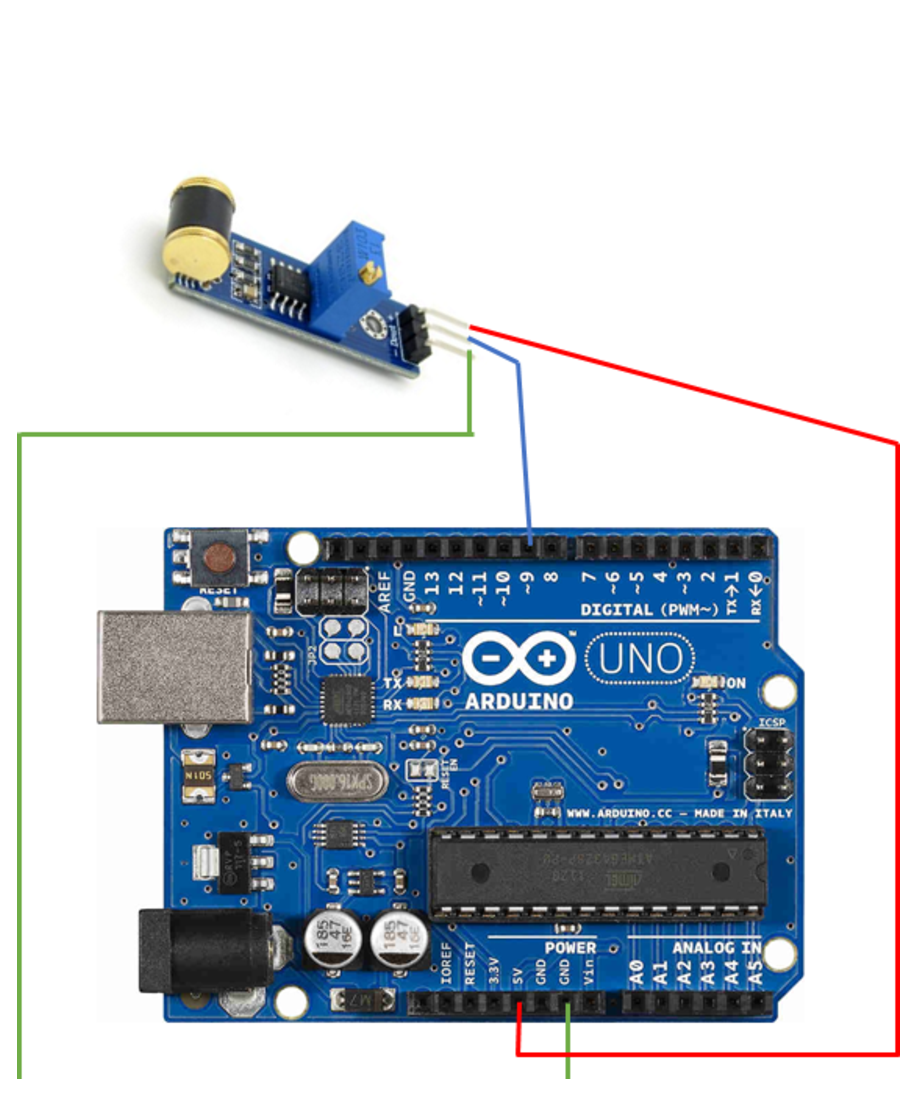
\includegraphics[scale=0.3]{ard2.eps}
	\item Connect the keypad as follows:\\
	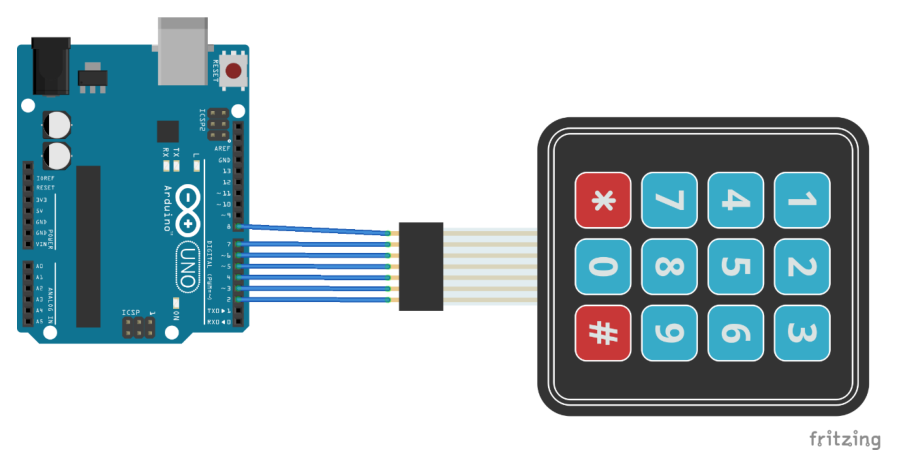
\includegraphics[scale=0.65]{ard1.eps}
	\item Connect the Ethernet shield on top of the board
	\item Plug a USB cable to the USB port (or the AC socket to a 5v power source).	
	\item Plug the netwrok RJ-45 cable to the Ethernet shield
\end{enumerate}
\subsection{Raspberry Pi}

\end{document}
